% !TEX root = 0-main.tex

\clearpage
\section*{Appendix}
\label{appendix}

\renewcommand\thefigure{\arabic{figure}}
\setcounter{figure}{1}      
\setcounter{section}{0}      

\renewcommand{\figurename}{Appendix Figure}

\section{Additional Discussions}
\subsection{FastPAM1 optimization}
\label{A2}

Algorithm \ref{alg:bandit_based_search} can also be combined with the FastPAM1 optimization from \cite{schubert2019faster} to reduce the number of computations in each SWAP iteration. 
For a given candidate swap $(m, x)$, we rewrite $g_{(m,x)}(x_j)$ from Eq. \eqref{eqn:swap_instance} as:
\begin{equation}
    \label{eqn:fastpam1-trick}
    g_{m,x}(x_j) = - d_1(x_j) + \mathbbm{1}_{x_j \notin \mathcal{C}_m}\min[d_1(x_j),d(x,x_j)] + \mathbbm{1}_{x_j \in \mathcal{C}_m}\min[d_2(x_j), d(x, x_j)]
\end{equation}
where $\mathcal{C}_m$ denotes the set of points whose closest medoid is $m$ and $d_1(x_j)$ and $d_2(x_j)$ are the distance from $x_j$ to its nearest and second nearest medoid, respectively, before the swap is performed. 
We cache the values $d_1(x_j), d_2(x_j)$, and the cluster assignments $\mathcal{C}_m$ so that Eq. \eqref{eqn:fastpam1-trick} no longer depends on $m$ and instead depend only on $\mathbbm{1}_{\{x_j \in \mathcal{C}_m \}}$, which is cached. This allows for an $O(k)$ speedup in each SWAP iteration since we do not need to recompute Equation \ref{eqn:fastpam1-trick} for each of the $k$ distinct medoids ($m$s).


\subsection{Value of re-estimating each \texorpdfstring{$\sigma_x$}{Lg}}
\label{A1}

% Allowing for arm-dependent $\sigma_x$ and re-estimating each $\sigma_x$ in each iteration also presents a difference between our approach and prior work {\bf \{citation\}}. Details about these techniques are discussed further in Section \ref{exps}. 


% We make the following additional changes to the vanilla version of Algorithm \ref{alg:bandit_based_search} to further improve speed. 

% The parameter $\sigma_x$ for the confidence intervals are estimated from data. Specifically, %\martin{Mo: could you add more information?}.
% We found that having different parameters for different steps of PAM will greatly improve speed. 
% We also found that the speed can be further improved by allowing a different parameter for different target points in $\mathcal{S}_{\text{tar}}$. 
% \martin{(As demonstrated in ...)}

\begin{figure}[h!]
    \centering
    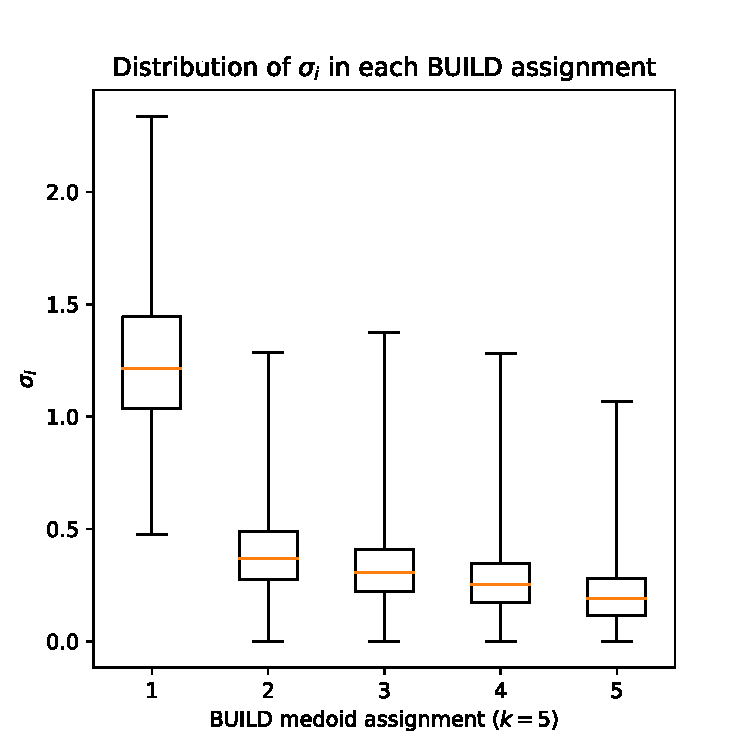
\includegraphics[scale=0.5]{figures/MNIST_sigmas_example.pdf}
    \caption{Boxplot showing the min, max, and each quartile for the set of all $\sigma_x$ estimates for the full MNIST dataset, in the BUILD step. } 
    \label{fig:MNIST_sigmas_example}
\end{figure}

The theoretical results in Section \ref{sec:theory} and empirical results in Section \ref{sec:exps} suggest that \algname scales almost linearly in dataset size for a variety of real-world datasets and commonly used metrics. One may also ask if Lines 7-8 of Algorithm \ref{alg:bandit_based_search}, in which we re-estimate each $\sigma_i$ from the data, are necessary.
In some sense, we treat the set of \{$\sigma_i$\} as adaptive in two different ways: $\sigma_i$ is calculated on a \textit{per-arm} basis (hence the subscript $i$), as well recalculated in each BUILD and SWAP iteration.
In practice, we observe that re-estimating each $\sigma_x$ for each sequential call to Algorithm \ref{alg:bandit_based_search} significantly improves the performance of our algorithm. Figure \ref{fig:MNIST_sigmas_example} describes the distribution of estimate $\sigma_x$ for the MNIST data at different stages of the BUILD step. The median $\sigma_x$ drops dramatically after the first medoid has been assigned and then steadily decreases, as indicated by the orange lines, and suggests that each $\sigma_x$ should be recalculated at every assignment step. Furthermore, the whiskers demonstrate significant variation amongst the $\sigma_x$ in a given assignment step and suggest that having arm-dependent $\sigma_x$ parameters is necessary. Without these modifications to our algorithm, we find that the confidence intervals used by \algname (Line 8) are unnecessarily large and cause computation to be expended needlessly as it becomes harder to identify good arms. Intuitively, this is due to the much larger confidence intervals that make it harder to distinguish between arms' mean returns.
For a more detailed discussion of the distribution of $\sigma_x$ and examples where the assumptions of Theorem \ref{thm:nlogn} are violated, we refer the reader to Appendix \ref{A3}.



\subsection{Violation of distributional assumptions}
\label{A3}

In this section, we investigate the robustness of \algname to violations of the assumptions in Theorem \ref{thm:nlogn} on an example dataset and provide intuitive insights into the degradation of scaling. We create a new dataset from the scRNA dataset by projecting each point onto the top 10 principal components of the dataset; we call the dataset of projected points scRNA-PCA. Such a transformation is commonly used in prior work; the most commonly used distance metric between points is then the $l_2$ distance \cite{scrnabestpractices}.

Figure \ref{fig:mu_dist} shows the distribution of arm parameters for various (dataset, metric) pairs in the first BUILD step. In this step, the arm parameter corresponds to the mean distance from the point (the arm) to every other point. We note that the true arm parameters in scRNA-PCA are more heavily concentrated about the minimum than in the other datasets. Intuitively, we have projected the points from a 10,170-dimensional space into a 10-dimensional one and have lost significant information in doing so. This makes many points appear "similar" in the projected space.

Figures \ref{fig:sigma_ex_MNIST} and \ref{fig:sigma_ex_SCRNAPCA} show the distribution of arm rewards for 4 arms (points) in MNIST and scRNA-PCA, respectively, in the first BUILD step. We note that the examples from scRNA-PCA display much larger tails, suggesting that their sub-Gaussianity parameters $\sigma_x$ are very high.

Together, these observations suggest that the scRNA-PCA dataset may violate the assumptions of Theorems \ref{thm:nlogn} and \ref{thm:specific} and hurt the scaling of \algname with $n$. Figure \ref{fig:SCRNAPCA-L2-scaling} demonstrates the scaling of \algname with $n$ on scRNA-PCA. The slope of the line of best fit is 1.204, suggesting that \algname scales as approximately $O(n^{1.2})$ in dataset size. We note that this is higher than the exponents suggested for other datasets by Figures \ref{fig:mods} and \ref{fig:scaling}, likely to the different distributional characteristics of the arm means and their spreads.

We note that, in general, it may be possible to characterize the distribution of arm returns $\mu_i$ at and the distribution of $\sigma_x$, the sub-Gaussianity parameter, at every step of \algnamenospace, from properties of the data-generating distribution, as done for several distributions in \cite{bagaria2018medoids}. We leave this more general problem, as well as its implications for the complexity of our \algname, to future work.

\begin{figure}[ht]
\begin{subfigure}{.5\textwidth}
  \centering
  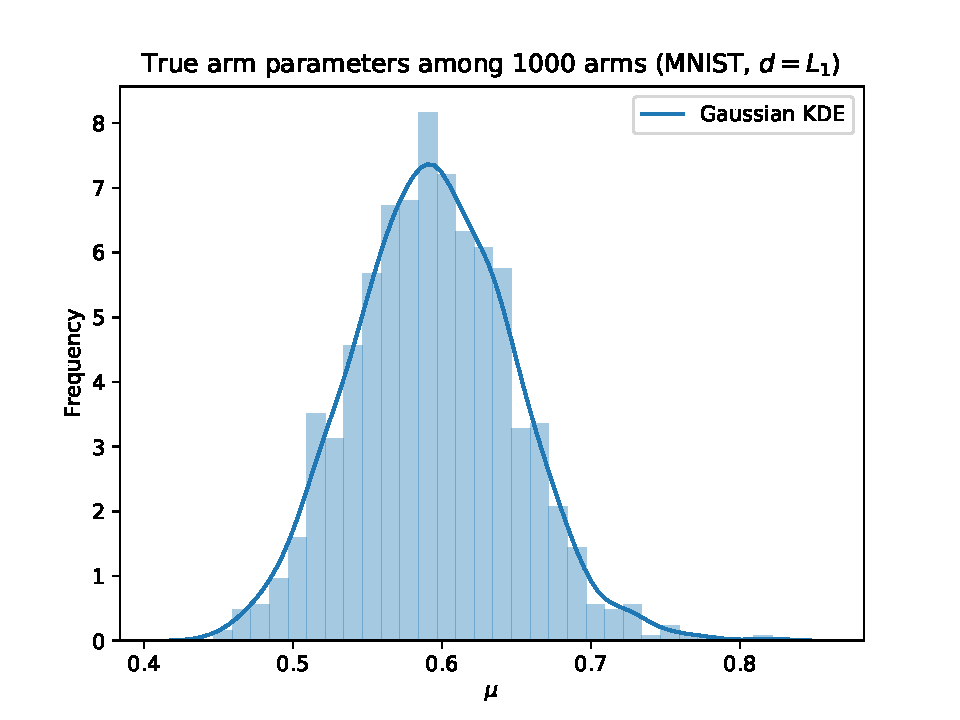
\includegraphics[width=\linewidth]{figures/mu-MNIST-COSINE.pdf}  
  \label{fig:mu_dist1}
\end{subfigure}
\begin{subfigure}{.5\textwidth}
  \centering
  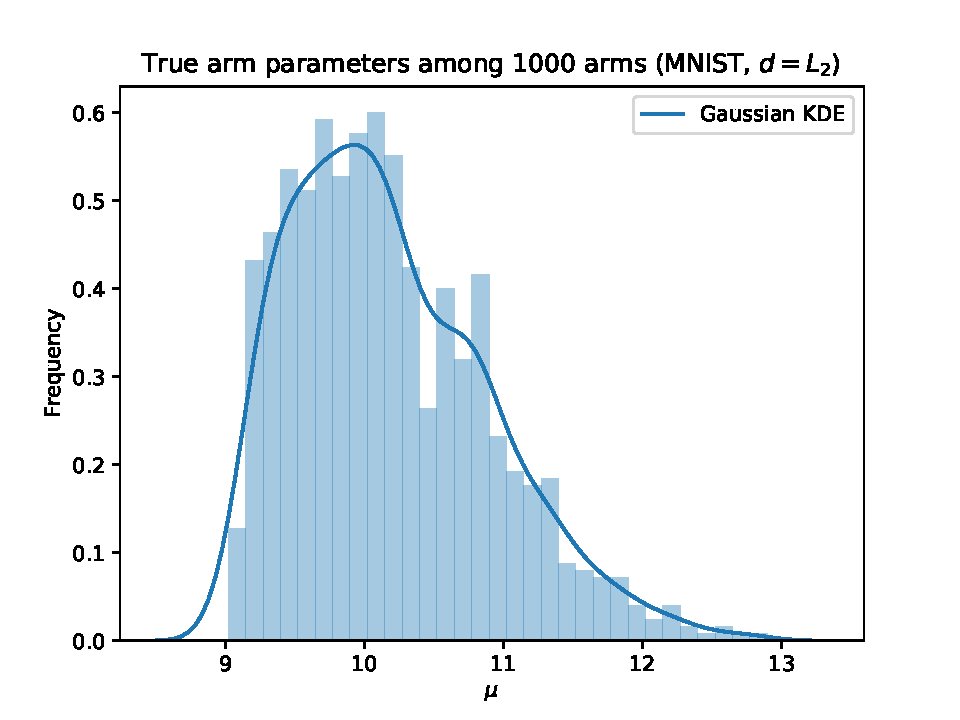
\includegraphics[width=\linewidth]{figures/mu-MNIST-L2.pdf}   
  \label{fig:mu_dist2}
\end{subfigure}
\begin{subfigure}{.5\textwidth}
  \centering
  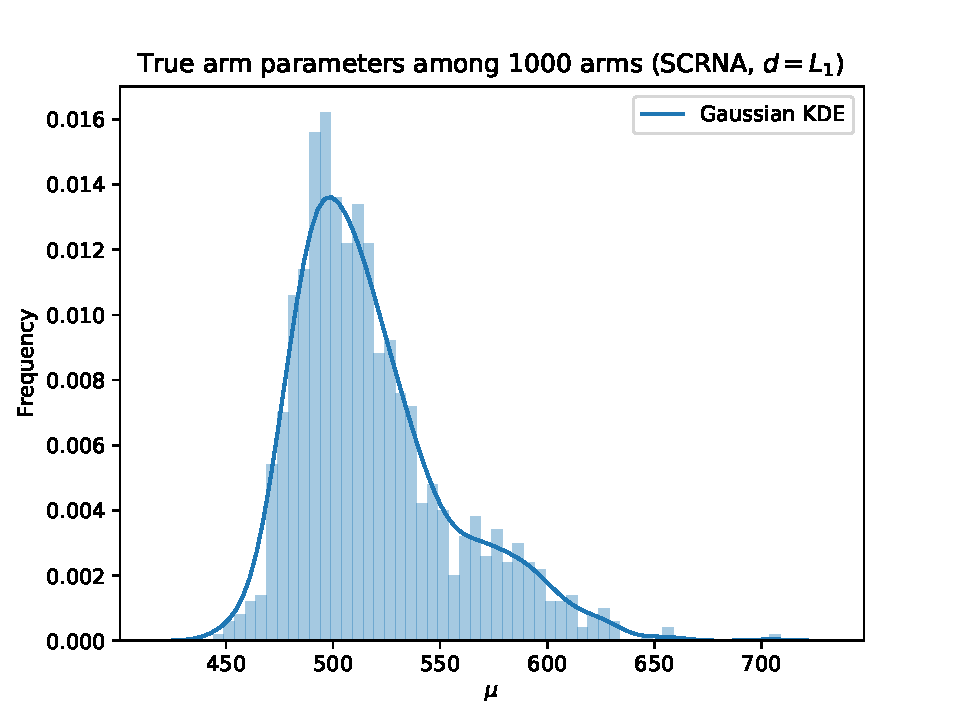
\includegraphics[width=\linewidth]{figures/mu-SCRNA-L1.pdf}   
  \label{fig:mu_dist3}
\end{subfigure}
\begin{subfigure}{.5\textwidth}
  \centering
  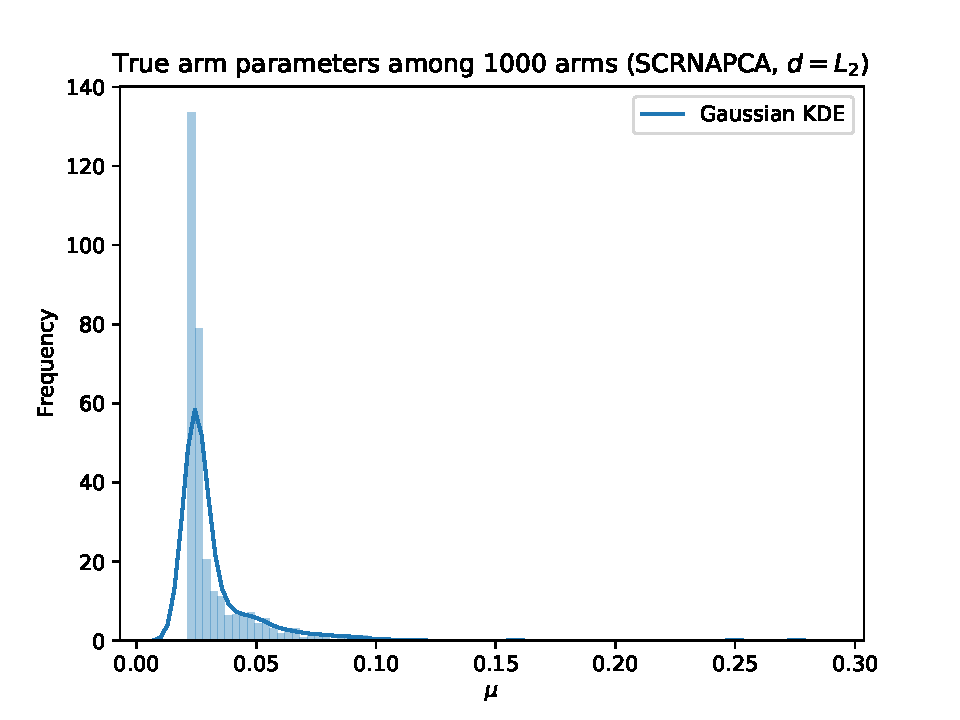
\includegraphics[width=\linewidth]{figures/mu-SCRNAPCA-L2.pdf}   
  \label{fig:mu_dist4}
\end{subfigure}
\caption{Histogram of true arm parameters, $\mu_i$, for 1000 randomly sampled arms in the first BUILD step of various datasets. For scRNA-PCA with $d = l_2$ (bottom right), the arm returns are much more sharply peaked about the mininum than for the other datasets. In plots where the bin widths are less than 1, the frequencies can be greater than 1.}
\label{fig:mu_dist}
\end{figure}

\begin{figure}[ht]
\begin{subfigure}{.5\textwidth}
  \centering
  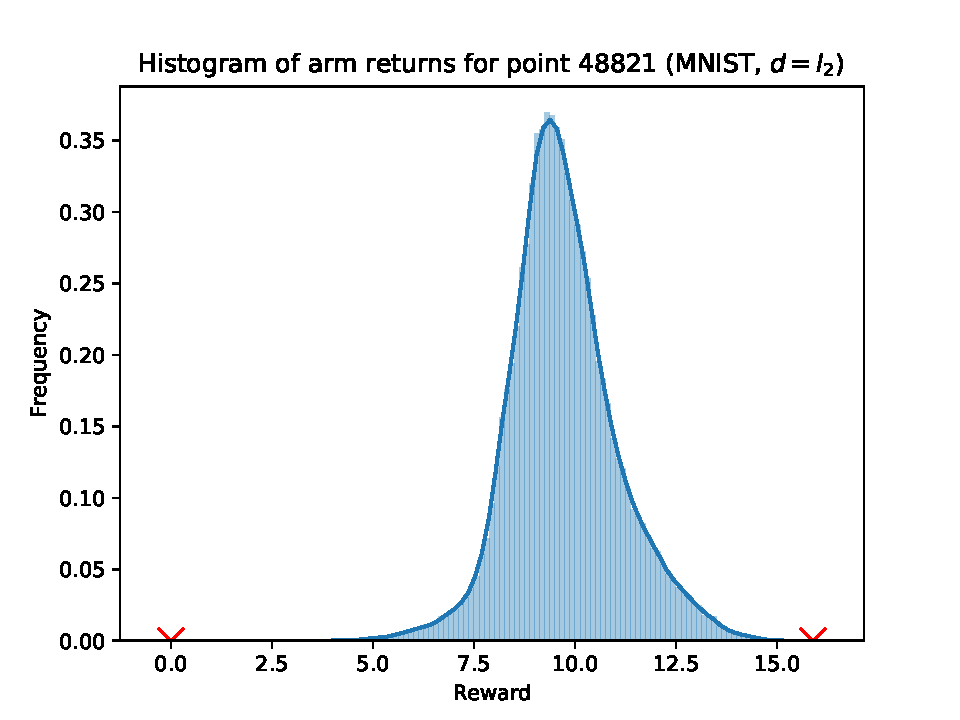
\includegraphics[width=\linewidth]{figures/sigma-MNIST-0-L2.pdf}  
\end{subfigure}
\begin{subfigure}{.5\textwidth}
  \centering
  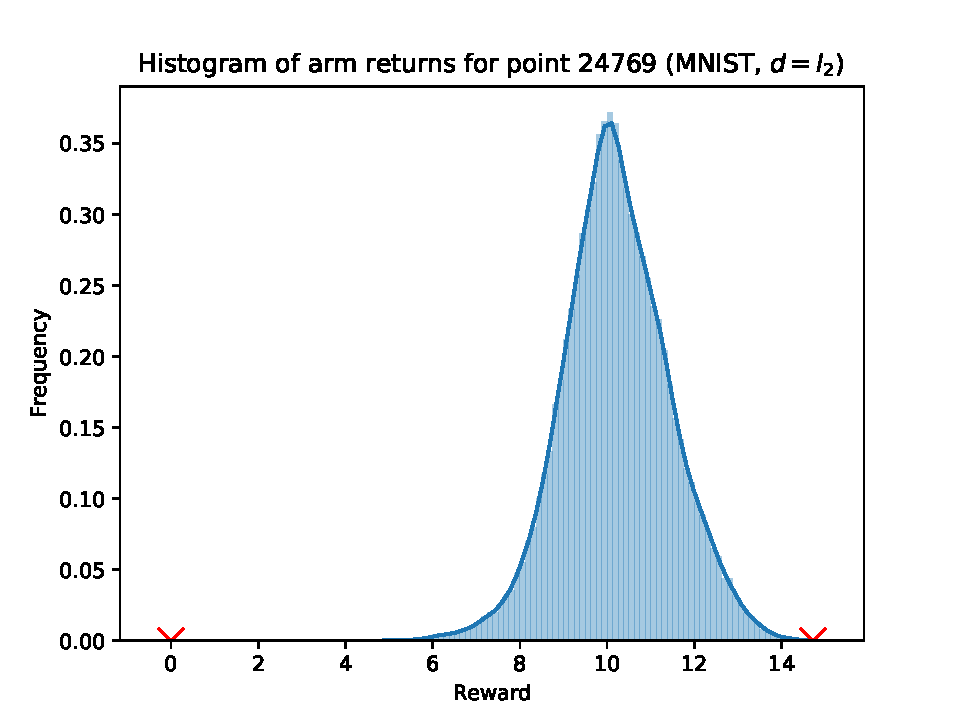
\includegraphics[width=\linewidth]{figures/sigma-MNIST-1-L2.pdf}   
\end{subfigure}
\begin{subfigure}{.5\textwidth}
  \centering
  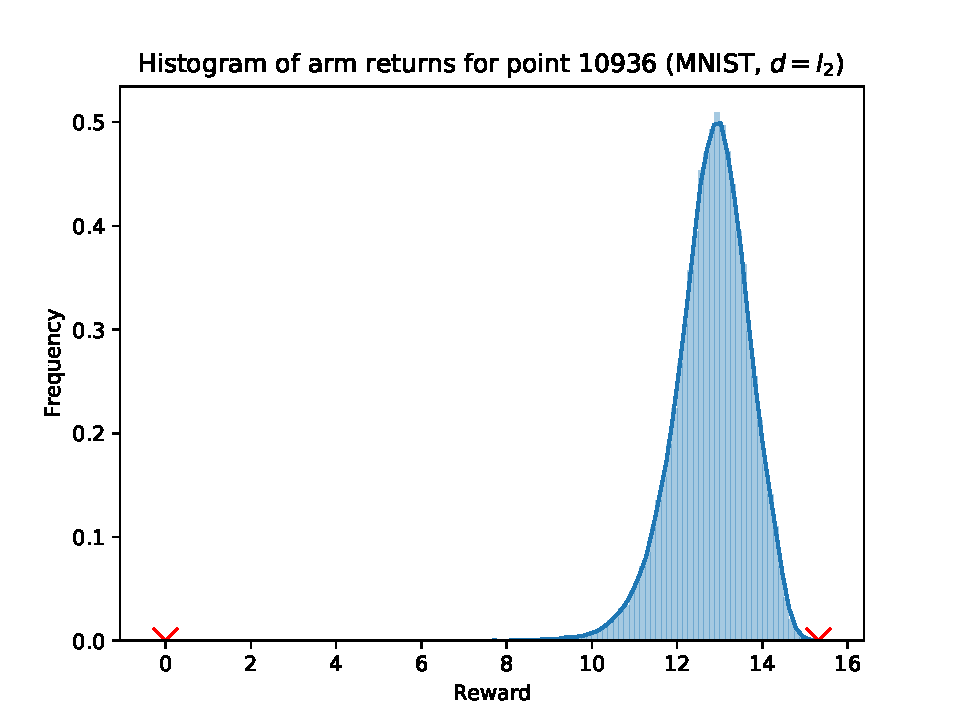
\includegraphics[width=\linewidth]{figures/sigma-MNIST-2-L2.pdf}   
\end{subfigure}
\begin{subfigure}{.5\textwidth}
  \centering
  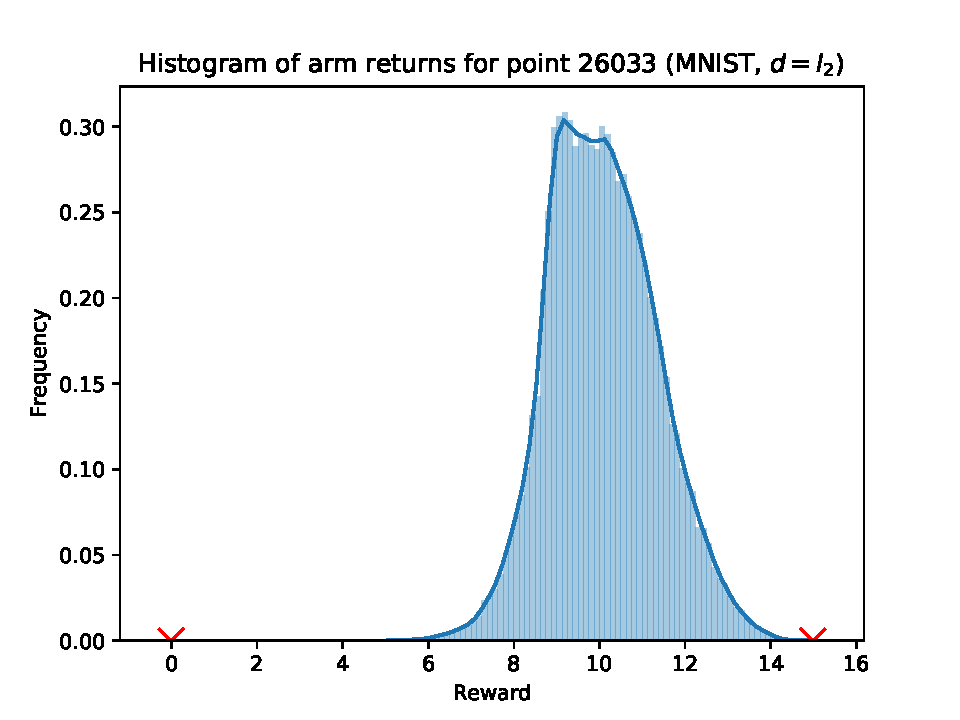
\includegraphics[width=\linewidth]{figures/sigma-MNIST-3-L2.pdf}   
\end{subfigure}
\caption{Example distribution of rewards for 4 points in MNIST in the first BUILD step. The minimums and maximums are indicated with red markers.}
\label{fig:sigma_ex_MNIST}
\end{figure}


\begin{figure}[ht]
\begin{subfigure}{.5\textwidth}
  \centering
  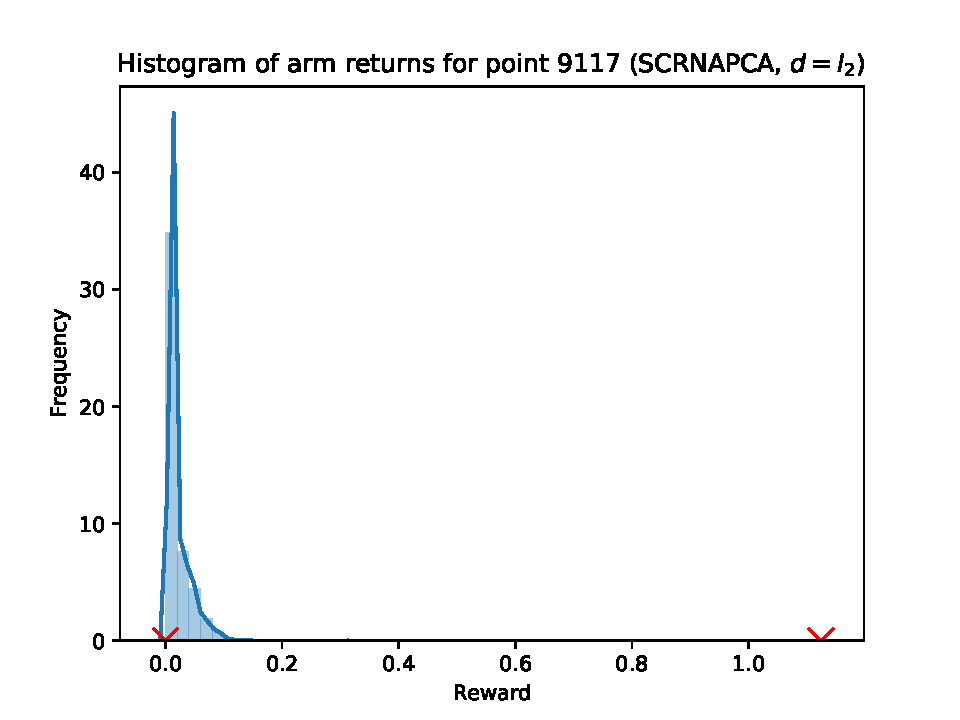
\includegraphics[width=\linewidth]{figures/sigma-SCRNAPCA-0-L2.pdf}  
\end{subfigure}
\begin{subfigure}{.5\textwidth}
  \centering
  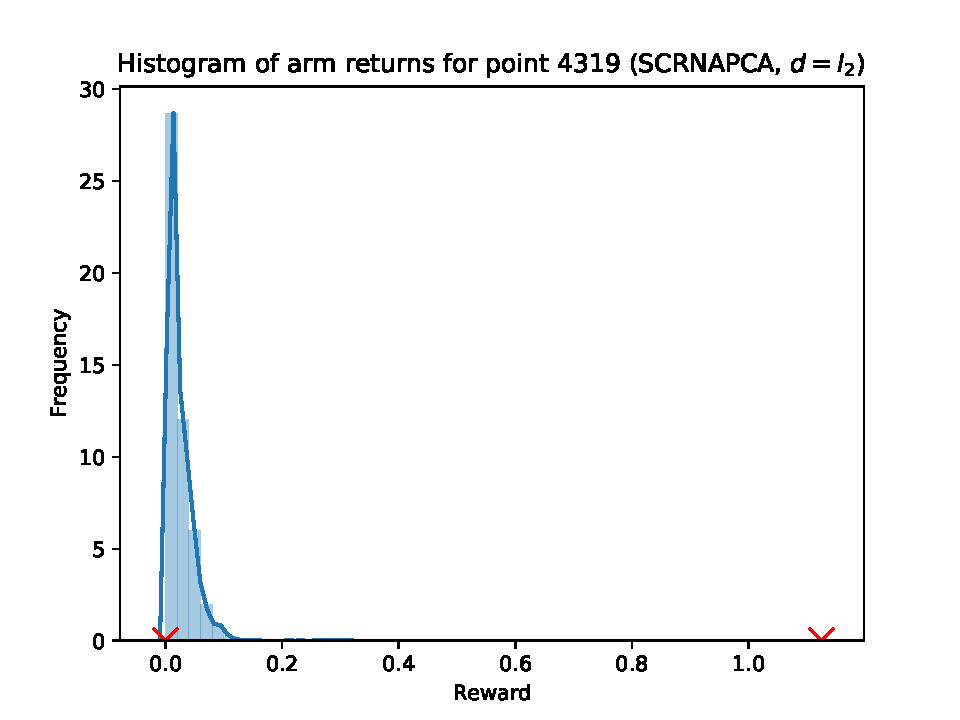
\includegraphics[width=\linewidth]{figures/sigma-SCRNAPCA-1-L2.pdf}   
\end{subfigure}
\begin{subfigure}{.5\textwidth}
  \centering
  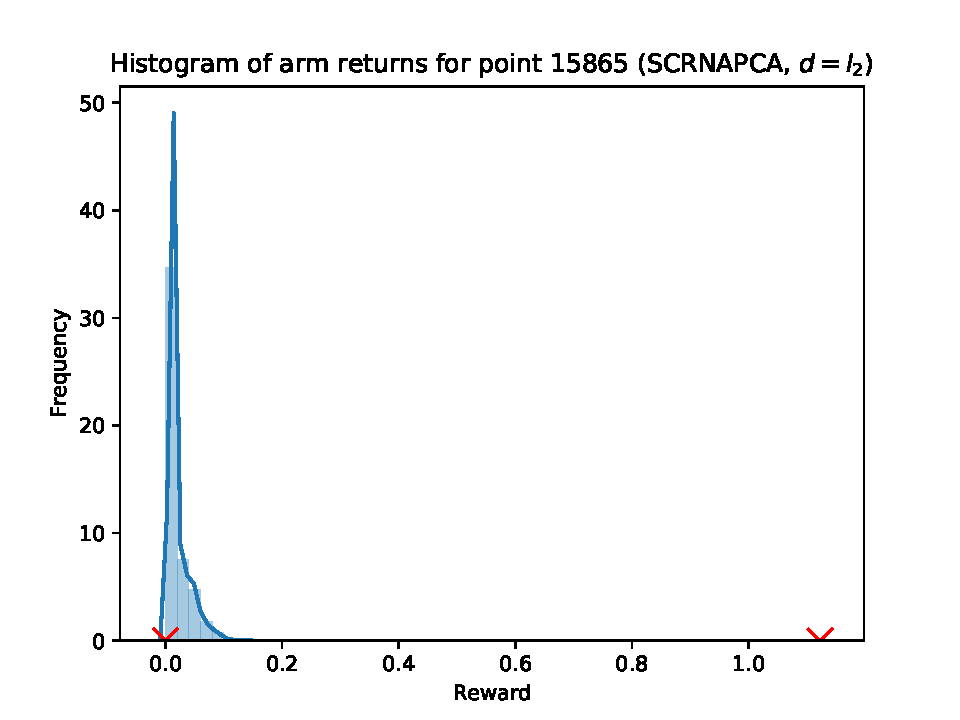
\includegraphics[width=\linewidth]{figures/sigma-SCRNAPCA-2-L2.pdf}   
\end{subfigure}
\begin{subfigure}{.5\textwidth}
  \centering
  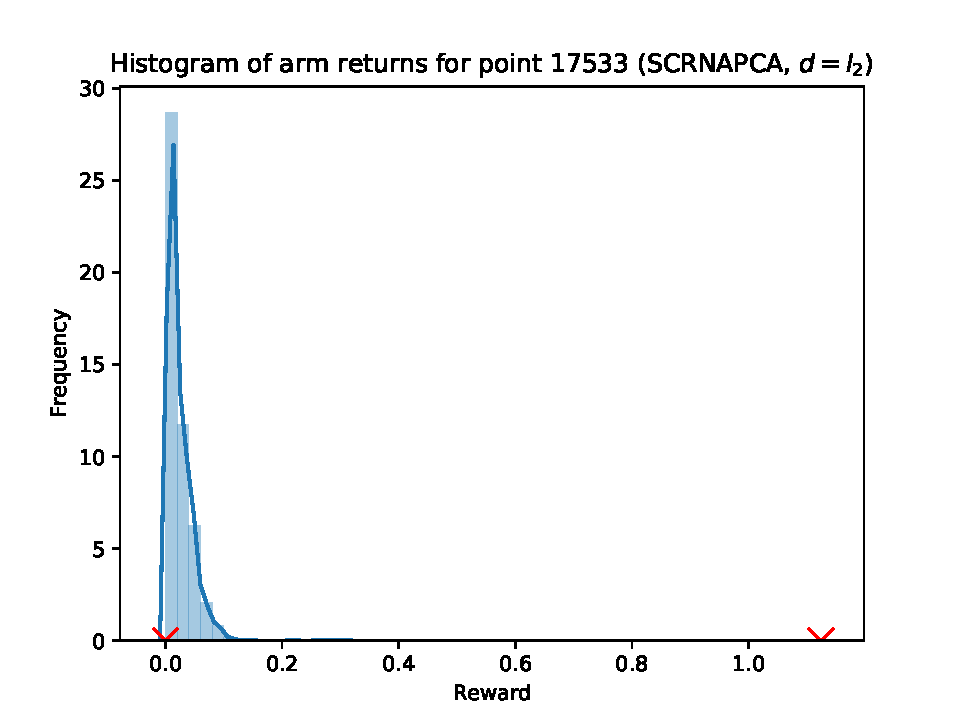
\includegraphics[width=\linewidth]{figures/sigma-SCRNAPCA-3-L2.pdf}   
\end{subfigure}
\caption{Example distribution of rewards for 4 points in scRNA-PCA in the first BUILD step. The minimums and maximums are indicated with red markers. The distributions shown here are more heavy-tailed than in Figure \ref{fig:sigma_ex_MNIST}. In plots where the bin widths are less than 1, the frequencies can be greater than 1.}
\label{fig:sigma_ex_SCRNAPCA}
\end{figure}


\begin{figure}[ht!]
    \centering
    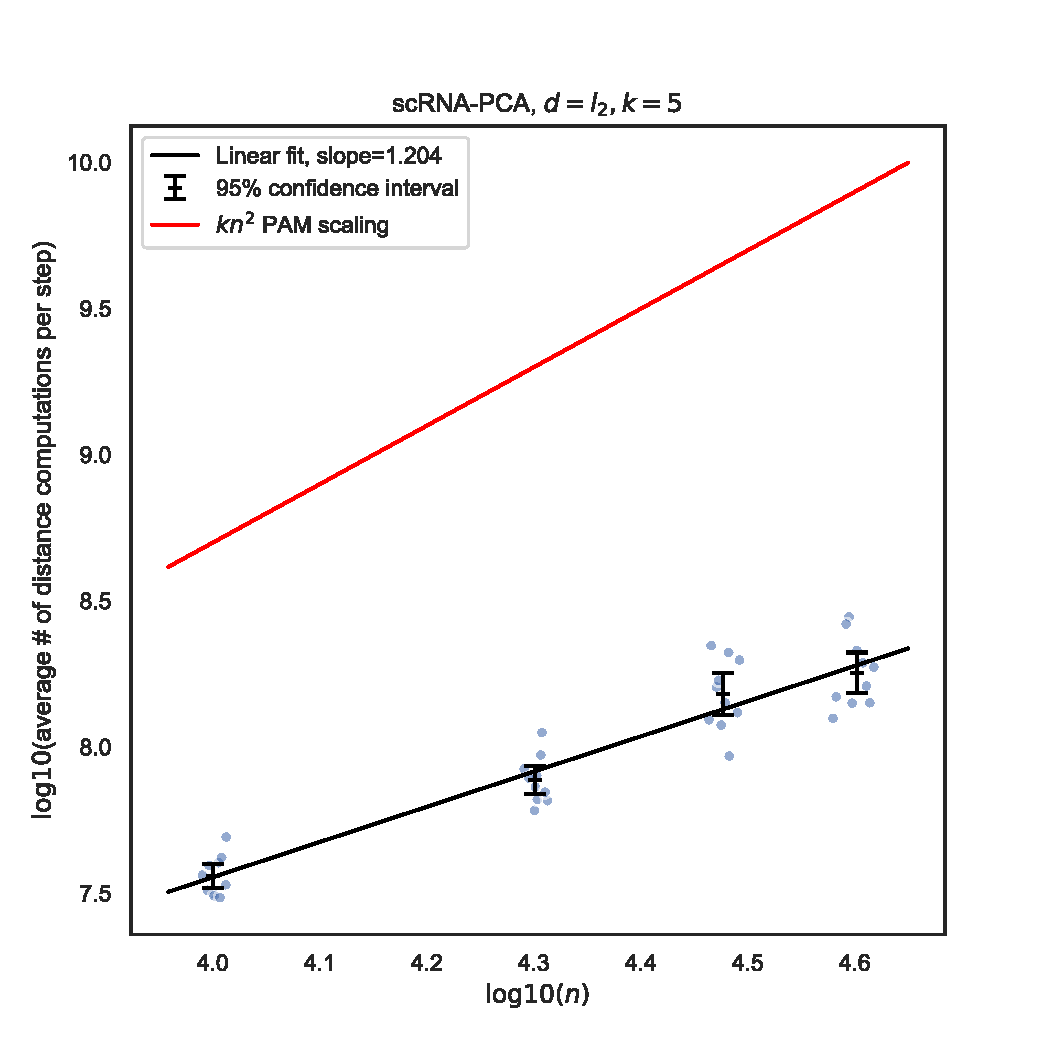
\includegraphics[scale=0.5]{figures/SCRNAPCA-L2-k5.pdf}
    \caption{Average number of distance calls per iteration vs $n$, for scRNA-PCA and $l_2$ distance on a log-log scale. The line of best fit (black) are plotted, as are reference lines demonstrating the expected scaling of PAM (red).} 
    \label{fig:SCRNAPCA-L2-scaling}
\end{figure}

\newpage
\clearpage
\section{Future Work}
\label{sec:future}
% \martin{Maybe move this section to Appendix}

% As part of this work, we developed and released a Python implementation of \algname. The runtime of our algorithms, as measured by wall time, could be significantly improved by reimplementing the algorithm in C++. In the future, we intend to release a high-performance C++ library for MAB-Based $k$-medoids algorithms, which could also be called from Python. Though we do not the theoretical complexity of the algorithm to differ amongst different language implementations, we can expect as large as a 20x improvement in wall time by reimplementing the algorithm in C++ \{citation\}.

% We also note that the PAM algorithm is used widely as a subroutine in several downstream algorithms, such as CLARA and CLARANS \{citation\}. \algname can be used as a modular "swap-in" for PAM these other algorithms, and would improve those algorithms' theoretical complexities and running times.

There are several ways in which \algname could be improved or made more impactful. In this work, we chose to implement a UCB-based algorithm to find the medoids of a dataset. Other best-arm-identification approaches, however, could also be used for this problem. 
%In particular, Thompson sampling may offer improvements over the UCB algorithm used here \{citation\}. 
An alternate approach using bootstrap-based bandits could also be valuable, especially in relaxing the distributional assumptions on the data that the quantities of interest are $\sigma$-sub-Gaussian \cite{wang2020bootstrap, kveton2019abootstrap, kveton2019bbootstrap}. It may also be possible to generalize a recent single-medoid approach, Correlation-Based Sequential Halving \cite{baharav2019ultra}, to more than 1 medoid. Though we do not have reason to suspect an algorithmic speedup (as measured by big-O), we may see constant factor improvements or improvements in wall clock time.

Throughout this work, we assumed that computing the distance between two points was an $O(1)$ operation. This obfuscates the dependence on the dimensionality of the data, $d$. If we consider computing the distance between two points an $O(d)$ computation, the complexity of \algname could be expressed as $O(dn$log$n)$ in the BUILD step and each SWAP iteration. Recent work \cite{bagaria2018adaptive} suggests that this could be further improved; instead of computing the difference in each of the $d$ coordinates, we may be able to adaptively sample which of the $d$ coordinates to use in our distance computations and reduce the dependence on dimensionality from $d$ to $O(\log d)$, especially in the case of sparse data.
%We note, however, that in practice most libraries contain software optimizations that make the dependence on $d$ for a distance computation sublinear (e.g. architecture optimizations); as such, we did not consider implementing this optimization in our work. 

% It is also important to note that the dissimilarity function used in the loss computation (Equation 1) is not required to be a distance metric; an arbitrary, even asymmetric, dissimilarity function could be used in more general settings.

Finally, it may be possible to improve the theoretical bounds presented in Theorem 1. We also note that it may be possible to prove the optimality of \algname in regards to algorithmic complexity, up to constant factors, using techniques from \cite{bagaria2018medoids} that were developed for sample-efficiency guarantees in hypothesis testing.

%Indeed, in our experiments, we found that \algname results agreed with PAM results with far more liberal error probability thresholds, $\delta$, than that suggested by Theorem 1, which allowed for better wall times. In fact, it may be possible to learn the "optimal" implementation parameters, such as $\delta$ and $\sigma$, directly from the data instead of empirically estimating them and treating them as constants. 


% Notes: Assuming sigma-sub-Guassian at the first step implies sigma-sub-Gaussian for later medoids. Do proof for k = 1 first and then induction.

% Let ${X_1, X_2, ..., X_N}$ each be $\sigma$-sub-Gaussian variables. Then, at the termination of the UCB algorithm when a new medoid is selected [i.e. lowest confidence interval is disjoint from others], we have that, for each $\mu_i$, with probability $1 - \delta$, $\mu_i \in [\hat{\mu_i} - C_i(t), \hat{\mu_i} + C_i(t)]$, where $C_i(t) = \sqrt{\frac{2\sigma^2log\frac{2}{\delta}}{T_i(t)}}$. Thus, with probability at least $1 - kN\delta$, the BUILD step of the UCB-based UltraPAM returns the same result as the BUILD step of PAM. Furthermore, if the original PAM algorithm takes $T$ SWAP steps to converge, then with probability  at least $1 - Tk(N-k)\delta$, the SWAP step of UltraPAM returns the same result as PAM. 

% Proof: At the termination of a single medoid assignment of the UltraPAM build step, the lowest confidence interval must be disjoint from all the other confidence intervals. Let the true medoid be point $1$ In order for an error to be made, at the end of the sampling, either $\hat{\mu_1}$ must be outside of its confidence interval or some other point (that will be incorrectly be chosen as the medoid) must be outside of its confidence interval [if none of these were true, we would not have an error -- crux of the argument]. By union bounding over the probability of any $\hat{\mu_i}$ not being in its confidence interval, we have:

% $P($Error in single BUILD assignment$) \leq N\delta$

% By union bounding this over all $k$ BUILD assignments, we have

% $P($Error in all BUILD$) \leq kN\delta$

% Thus, with probability at least $1 - kN\delta$, the BUILD step of UltraPAM chooses the same initial $k$ medoids as PAM.

% Pf. Similar to above, but with $T$ iterations and $k(N-k)$ arms. So error is 

% $P($Error in all SWAP$) \leq Tk(N-k)\delta$



% Note: define consistency as agreeing with PAM.

% 1. Best-arm identification
% 2. Same results as PAM
% 3. Number of swap steps
% 4. Quantify how often fallback occurs


% % \begin{algorithm}[t]
% %   \caption{\texttt{Med-dit} \label{alg:UCB-Medoid}}
% %   \label{alg:cpca1}
% % \begin{algorithmic}[1]
% %   \STATE Evaluate 
% %   distances 
% %   of each point to a randomly 
% %   chosen point and build a $(1-\delta)$-confidence interval
% %   for the mean distance 
% %   of each point $i$:
% %   $[\hat{\mu}_i(1)-C_i(1), \ \hat{\mu}_i(1)+C_i(1)]$.    
% %   \WHILE \TRUE
% %   \STATE At iteration $t$, pick point $A_t$ that 
% %   minimises $\hat{\mu}_i(t-1)-C_i(t-1)$.    
% %     \IF{distances of point $A_t$ are 
% %   evaluated less than $n-1$ times}
% %     \STATE evaluate the distance
% %   of $A_t$ to a randomly picked point 
% %   and update the confidence interval of $A_t$.
% %     \ELSE
% %     \STATE Set 
% %   $\hat{\mu}_i(t)$ to be the empirical mean 
% %   of distances of point $A_t$ by 
% %   computing its distance to all $(n-1)$ other
% %   points and set 
% %   $C_{A_t}(t)=0$.
% %   \ENDIF
% %   \IF {there exists a point $x_{i^*}$ 
% %   such that $\forall  i\neq i^*$, 
% %   $\hat{\mu}_{i^*}(t) + C_{i^*}(t) < \hat{\mu}_i(t) - C_i(t)$}
% %     \RETURN $x_{i^*}$.
% %   \ENDIF  
% %   \ENDWHILE
% % \end{algorithmic}
% % \end{algorithm}




% %%% For use with ALGORITHMC package
% % \begin{algorithm}[t]
% % \caption{\texttt{UltraPAM\_BUILD($X, k_{max}, d$):} \label{alg:ultrapam-build}}

% % \begin{algorithmic}[1]
% %     \FOR{$k = 1, 2, ..., k_{max}$}
% %     \STATE $\mathcal{M} = \emptyset$
% %     \STATE $arms \leftarrow [n]$
% %     \STATE $T \leftarrow (0, \dots, 0)$
% %     \STATE $L, M, U = (-\infty, \dots, -\infty), (0, 0, 0), (\infty, \dots, \infty)$
% %         \WHILE{$arms \neq \emptyset$}
% %             % Question: should we even include this case in the pseudocode?
% %             \FORALL{arms $i$ that have been sampled more than $N$ times} \STATE Compute $\sum_{x_{\rm ref}}\Delta TD_{x_i}(x_{\rm ref})$ exactly
% %             \STATE Set $L_i = M_i = U_i = \sum_{x_{\rm ref}}\Delta TD_{x_i}(x_{\rm ref})$
% %             \ENDFOR
            
% %             \FORALL{arms $i$ that have been sampled less than $N$ times}
% %             \STATE Sample a reference point $x_{\rm ref}$ uniformly at random 
% %             \STATE $means_i \leftarrow \frac{ T_imeans_i + \Delta TD_{x_i}(x_{\rm ref})}{T_i + 1}$
% %             \STATE $C_i \leftarrow \sigma \sqrt{ \frac{ log(\frac{1}{\delta}) } {T_i}}$
% %             \STATE $L_i \leftarrow means_i - C_i$
% %             \STATE $U_i \leftarrow means_i + C_i$
% %             \STATE $T_i \leftarrow T_i + 1$
% %             \ENDFOR

% %         \STATE $arms \leftarrow \{i : L_i \leq \min_i(U_i)\}$
% %         \ENDWHILE
% %         \STATE Append $x_i$ to $\mathcal{M}$, where $i = \argmin_iL_i$
% % \ENDFOR
% % \RETURN $\mathcal{M}$
% % \end{algorithmic}
% % \end{algorithm}





% ...thus converting the double sum to a MAB problem... 
% Need to specify k << N


% % \section{Figures and Tables}
% % \subsection{Figures}

% % \begin{figure}
% %   \centering
% %   \fbox{\rule[-.5cm]{0cm}{4cm} \rule[-.5cm]{4cm}{0cm}}
% %   \caption{Sample figure caption.}
% % \end{figure}

% % \subsection{Tables}

% % \begin{table}
% %   \caption{Sample table title}
% %   \label{sample-table}
% %   \centering
% %   \begin{tabular}{lll}
% %     \toprule
% %     \multicolumn{2}{c}{Part}                   \\
% %     \cmidrule(r){1-2}
% %     Name     & Description     & Size ($\mu$m) \\
% %     \midrule
% %     Dendrite & Input terminal  & $\sim$100     \\
% %     Axon     & Output terminal & $\sim$10      \\
% %     Soma     & Cell body       & up to $10^6$  \\
% %     \bottomrule
% %   \end{tabular}
% % \end{table}



\clearpage
\section{Proof of Theorem~\ref{thm:specific}}
\label{app:thmproof}


% \begin{proof}[Proof of Theorem~\ref{thm:specific}]


% Notice that, if more than $n$ distance computations are performed for a given arm $x$, the algorithm abandons the current estimate $\hat L_x$ and computes $\bar L_x$ exactly (which requires additional $n$ computations), setting $C_x = 0$.
% This guarantees that the algorithm must terminate.
% At the end, for arm $x$, the total number of distance computations will be either $T_x$ or $2n$. % if $T_x = n$.
\begin{proof}
First, we show that, with probability $1-\tfrac{2}{n}$, all confidence intervals computed throughout the algorithm are true confidence intervals, in the sense that they contain the true parameter $\mu_x$.
% \mo{need to be more explicit about what is "true" CI}
To see this, notice that for a fixed $x$ and a fixed iteration of the algorithm, $\hat \mu_x$ is the average of $\nuref$ i.i.d.~samples of a $\sigma_x$-sub-Gaussian distribution.
From Hoeffding's inequality, 
\aln{
\Pr\left( \left| \mu_x - \hat \mu_x \right| > C_x \right) \leq 2 \exp \left({-\frac{\nuref C_x^2}{2\sigma_x^2}}\right)  = 2 \delta.
% \\
% \sigma_x \sqrt{ \frac{2 \log(\frac{1}{\delta}) } {T_x}}
}
Notice that there are at most $n^2/\batchsize \leq n^2$ such confidence intervals computed across all target points (i.e., arms) and all steps of the algorithm.
If we set $\delta = 1/n^3$, we see that $\mu_x \in [\hat \mu_x - C_x, \hat \mu_x + C_x]$ for every $x$ and for every step of the algorithm with probability at least $1-2/n$, by the union bound.

Let $x^* = \argmin_{x \in \Star} \mu_x$.
Notice that if all confidence intervals throughout the algorithm are correct, it is impossible for $x^*$ to be removed from the set of candidate target points. 
Moreover, it is clear that the main while loop in the algorithm can only run $n/\batchsize$ times and that the algorithm must terminate.
Hence, $x^*$ (or some $y \in \Star$ with $\mu_y = \mu_{x^*}$) must be returned upon termination.


% Now consider a suboptimal arm $x \ne x^*$. 
Let $\nuref$ be the total number of arm pulls computed for each of the arms remaining in the set of candidate arms at some point in the algorithm.
Notice that, for any suboptimal arm $x \ne x^*$ that has not left the set of candidate arms, we must have
$C_x = \sigma_x \sqrt{ 2 \log(\tfrac{1}{\delta}) /\nuref}$.
% Hence, if $N$
Moreover, if $\nuref > \frac{24}{\Delta_x^2} \left(\sigma_x+\sigma_{x^*}\right)^2 \log n$,
% if $N > (24 \sigma_x^2 \log n)/(\Delta_x^2 \sigma_{x^*}^2) \log n$, 
we have that
\aln{
2(C_x + C_{x^*}) = 2 \left( \sigma_x + \sigma_{x^*}\right) \sqrt{  { 2 \log(n^3) } / {\nuref  }} < \Delta_x = \mu_x - \mu_{x^*},
}
and 
$
\hat \mu_x - C_x > \mu_x - 2C_x = \mu_{x^*} + \Delta_x - 2C_x 
\geq \mu_{x^*} + 2 C_{x^*} > \hat \mu_{x^*} + C_{x^*},
$
% \aln{
% \hat L_x - C_x & > \bar L_x - 2C_x = \bar L_{x^*} + \Delta_x - 2C_x 
% = \bar L_{x^*} + \Delta_x - {2\sigma_x} \sqrt{  2 \log(n^3) / N } \\
% & > \bar L_{x^*} + \Delta_x - {2\sigma_x} \Delta_x \frac{ \sigma_x }{2 + \sigma_{x^*}} = 
% \\
% & \geq \bar L_{x^*} + 2 C_{x^*} = \hat L_{x^*} + C_{x^*},
% }
implying that $x$ must be removed from the set of candidate arms at the end of that iteration.
Hence, the number of distance computations $M_x$ required for target point $x \ne x^*$ is at most
\aln{
M_x \leq \min \left[ \frac{24}{\Delta_x^2} \left( \sigma_x + \sigma_{x^*}\right)^2 \log n + \batchsize, 2n \right].
}
Notice that this holds simultaneously for all $x \in \Star$ with probability $1-\tfrac{2}{n}$.
We conclude that the total number of distance computations $M$ satisfies
\aln{
E[M] & \leq E[M | \text{ all confidence intervals are correct}] + \frac{2}{n} (2n^2) \\
& \leq 4n + \sum_{x \in \X}  \min \left[ \frac{24}{\Delta_x^2} \left( \sigma_x + \sigma_{x^*}\right)^2 \log n + \batchsize, 2n \right],
}
where we used the fact that the maximum number of distance computations per target point is $2n$.
% , if the confidence intervals are not all correct throughout the algorithm, which occurs with probability at most $\tfrac2\delta$, then we may use at most $2n$ computations per target point.
\end{proof}
